\documentclass[11pt,a4paper]{article}
\usepackage[utf8]{inputenc}
\usepackage[T1]{fontenc}
\usepackage{tgpagella}
\usepackage[spanish]{babel}
\usepackage{geometry}
\usepackage{booktabs}
\usepackage{xcolor}
\usepackage{titlesec}
\usepackage{fancyhdr}
\usepackage[parfill]{parskip}
\usepackage[expansion=false]{microtype}
\usepackage{hyperref}
\usepackage{setspace}
\usepackage{needspace}
\usepackage{graphicx}
\widowpenalty=10000
\clubpenalty=10000
\displaywidowpenalty=10000

\geometry{top=3.0cm,bottom=3.0cm,left=3.5cm,right=3.5cm}
\setlength{\parskip}{0.65em}
\setlength{\parindent}{0em}

\definecolor{azulai}{RGB}{30,80,140}
\definecolor{doradoai}{RGB}{140,90,0}
\definecolor{grisai}{RGB}{70,70,70}

\titleformat{\section}{\Large\bfseries\color{azulai}}{}{0em}{}[{\color{azulai}\titlerule[0.5pt]}]
\titlespacing*{\section}{0pt}{1.8em}{0.8em}
\titleformat{\subsection}{\large\bfseries\color{doradoai}}{}{0em}{}
\titlespacing*{\subsection}{0pt}{1.4em}{0.5em}
\titleformat{\subsubsection}{\normalsize\bfseries\color{grisai}}{}{0em}{}
\titlespacing*{\subsubsection}{0pt}{1.0em}{0.3em}

\pagestyle{fancy}\fancyhf{}
\rhead{\textcolor{grisai}{\small Amaya Beatriz — Arquitectura Interna}}
\lhead{\textcolor{grisai}{\small Sol · Ascendente · Nodos}}
\cfoot{\textcolor{grisai}{\small\thepage}}
\renewcommand{\headrulewidth}{0.3pt}

\hypersetup{colorlinks=true,linkcolor=azulai,urlcolor=azulai}
\setstretch{1.45}
\tolerance=1500
\emergencystretch=4em

\begin{document}

% ── Portada ──────────────────────────────────────────────────────────────────
\begin{titlepage}
  \centering
  \vspace*{1.5cm}
  {\Huge\bfseries\color{azulai} Sol · Ascendente · Nodos}\\[0.5cm]
  {\large\color{grisai} Arquitectura Interna}\\[0.3cm]
  {\small\itshape\color{grisai} Dirección vital, punto de entrada y eje de desarrollo}\\[2cm]
  {\huge\color{doradoai} Amaya Beatriz}\\[1.5cm]
  {\Large 30/10/1976 \quad 22:10}\\[0.3cm]
  {\Large Zaragoza, España}\\[0.3cm]
  {\normalsize Lat: 41.6916° \quad Lon: -0.9101° \quad UTC+01:00}\\[0.3cm]
  {\normalsize Ascendente: Cáncer 16°08' \quad
    MC: Piscis 25°32'}\\[2cm]
  \begin{tabular}{lll}
    \textbf{Sol:} & Escorpio & Casa 5 \\
    \textbf{Ascendente:} & Cáncer & Punto de entrada principal: la Luna \\
    \textbf{Nodo Norte:} & Escorpio & Casa 5 \\
    \textbf{Nodo Sur:}   & Tauro & Casa 11 \\
  \end{tabular}\\[2cm]
  \vfill
  {\small Generado el 19/05/2026}
\end{titlepage}

\tableofcontents
\newpage

% ── Datos de referencia ───────────────────────────────────────────────────────
\section{Datos de referencia}

\begin{center}
\begin{tabular}{llll}
  \toprule
  \textbf{Punto} & \textbf{Signo} & \textbf{Casa} & \textbf{Posición} \\
  \midrule
  Sol           & Escorpio & 5 & 7°35' \\
  Ascendente    & Cáncer & --- & 16°08' \\
  Medio Cielo   & Piscis & --- & 25°32' \\
  Nodo Norte    & Escorpio & 5 & 3°33' \\
  Nodo Sur      & Tauro & 11 & 3°33' \\
  \bottomrule
\end{tabular}
\end{center}

\vspace{0.5cm}
\textbf{Regente del Ascendente (Cáncer):} 
la Luna —
, 
Casa 

\vspace{0.5cm}
\textbf{Aspectos entre Sol, Ascendente y Nodos:}

\begin{center}
\begin{tabular}{lllll}
  \toprule
  \textbf{Planeta 1} & \textbf{Asp.} & \textbf{Planeta 2} & \textbf{Tipo} & \textbf{Orbe} \\
  \midrule
  Sol & = & Nodo Norte & Conjunción & 4.0° \\
  Sol & ☍ & Nodo Sur & Oposición & 4.0° \\
  \bottomrule
\end{tabular}
\end{center}

\needspace{3\baselineskip}
\subsection*{Grados sensibles}



\vspace{0.7cm}

\begin{center}
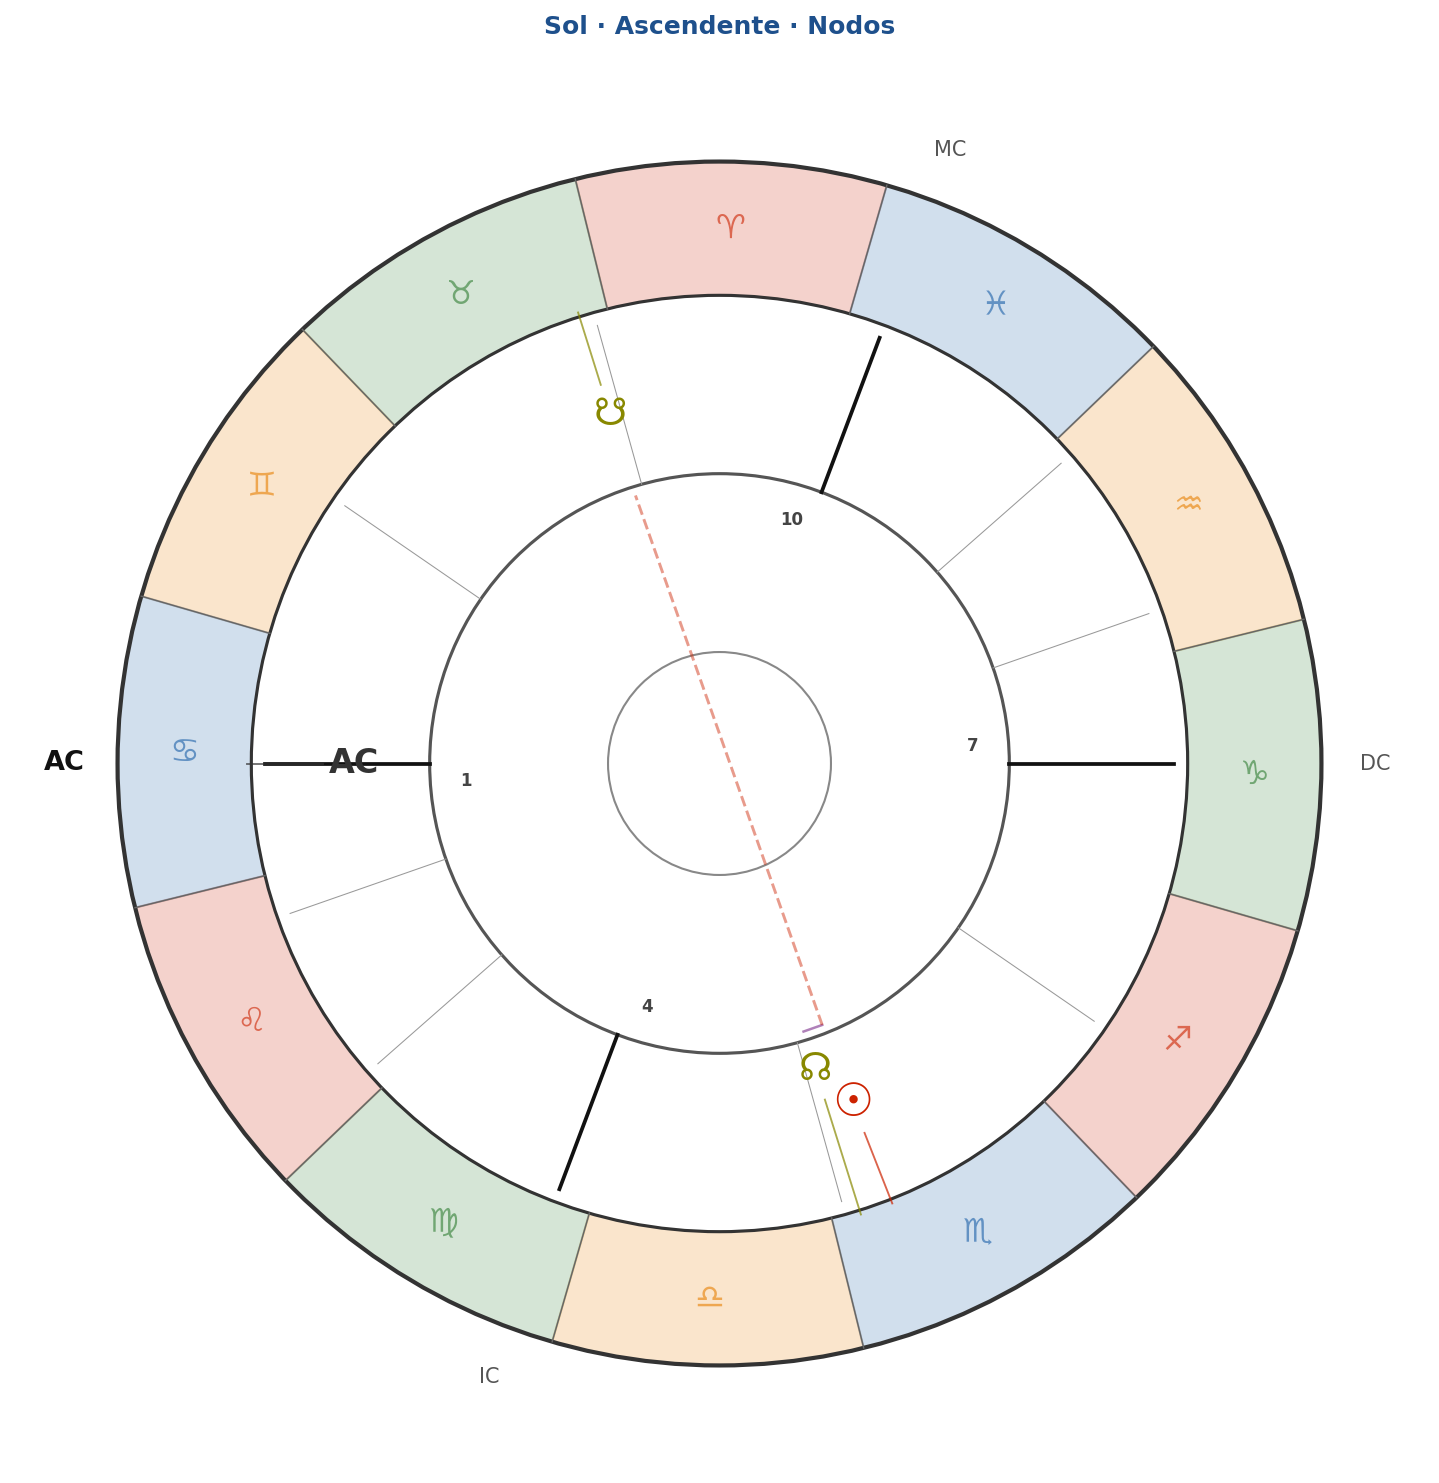
\includegraphics[width=0.72\textwidth]{Amaya_Beatriz_Sol_ASC_Nodos_rueda.png}
\end{center}


\vspace{0.3cm}
\Needspace{5\baselineskip}

% ── Interpretación ────────────────────────────────────────────────────────────
\section{Interpretación — Arquitectura Interna}

\begin{center}
{\small\itshape
No se trata de definir quién eres. Se trata de observar cómo se organiza tu dirección,
cómo atraviesas la vida y qué tensión influye en tu forma de avanzar.
}
\end{center}

\vspace{0.5cm}
\Needspace{5\baselineskip}


% ── 1. Dirección general ──────────────────────────────────────────────────────
\needspace{3\baselineskip}
\subsection{1. Dirección general}

El Sol está en Escorpio, Casa 5. El Ascendente está en Cáncer. El Nodo Norte está en Escorpio, Casa 5, y el Nodo Sur en Tauro, Casa 11.

El Sol en Escorpio y el Ascendente en Cáncer pertenecen al mismo elemento. Esto suele hacer que la forma en la que vives la vida y tu dirección principal estén bastante alineadas.

El Sol y el Nodo Norte están en Escorpio. Esto une tu dirección principal con una zona importante de crecimiento. Puede haber una sensación más clara de hacia dónde avanzar, aunque eso no significa que el trabajo ya esté hecho.

\vspace{0.5cm}
\Needspace{5\baselineskip}


% ── 2. Sol ────────────────────────────────────────────────────────────────────
\needspace{3\baselineskip}
\subsection{2. El Sol — Dirección principal}

\needspace{3\baselineskip}
\subsubsection*{Sol en Escorpio · Casa 5}

Tu dirección se activa cuando sientes que hay algo verdadero en juego. Necesitas profundidad, intensidad y contacto con lo que transforma de verdad.

Las dinámicas superficiales o vacías suelen agotarte rápidamente. Cuando no encuentras profundidad en lo que haces, puedes acabar controlándolo todo, desconfiando o acumulando tensión por dentro.

Te afecta mucho la traición, la pérdida de confianza o sentir que no puedes transformar algo importante en tu vida. Cuando la energía no encuentra salida, puede volverse contra ti en forma de obsesión, desgaste o bloqueo emocional.

Tu dirección se activa cuando puedes crear, expresar o aportar algo propio. Necesitas sentir que hay una parte auténtica de ti en lo que haces.

Los espacios demasiado impersonales o donde no puedes dejar huella suelen apagarte poco a poco. También te afecta mucho sentir que lo que haces no importa o pasa desapercibido.

Cuando puedes jugar, crear o implicarte de verdad en algo, recuperas rápidamente energía y claridad.

El Sol y el Nodo Norte apuntan hacia la misma dirección. Existe una sensación más natural de avanzar hacia aquello que necesitas desarrollar y muchas veces ciertas decisiones importantes se sienten coherentes internamente incluso cuando requieren esfuerzo o implican atravesar incomodidad. La dirección suele percibirse con más claridad que en otras configuraciones y puede existir sensación de que algunas experiencias importantes encajan profundamente con lo que necesitas construir. El reto está en no confundir facilidad con trabajo ya realizado. A veces el crecimiento parece tan natural que cuesta ver cuándo sigues funcionando desde patrones antiguos o demasiado conocidos.

El Sol se opone al Nodo Sur y apunta hacia el Nodo Norte. La dirección de crecimiento suele sentirse mucho más visible y alineada con tu impulso vital y con aquello que necesitas construir hacia adelante. Aun así, el Nodo Sur continúa funcionando como un lugar de regreso automático en momentos de cansancio, miedo o exceso de presión. Lo antiguo sigue teniendo fuerza aunque ya no sea el lugar principal de desarrollo. El reto está en no idealizar únicamente la dirección de crecimiento olvidando que también necesitas comprender y ordenar aquello que dejas atrás.


\vspace{0.5cm}
\Needspace{5\baselineskip}


% ── 3. Ascendente ─────────────────────────────────────────────────────────────
\needspace{3\baselineskip}
\subsection{3. El Ascendente — Forma de relacionarte con la vida}

\needspace{3\baselineskip}
\subsubsection*{Cáncer · Regente: la Luna}

Tu primera reacción suele ser percibir si hay seguridad o no en lo que está ocurriendo. Antes incluso de pensarlo, tu cuerpo ya está leyendo el ambiente y evaluando cuánto puede relajarse.

Cuando no sientes seguridad o el entorno es ambiguo, es fácil cerrarte, protegerte o tomar distancia aunque sigas presente hacia afuera.

Necesitas espacios donde puedas bajar la guardia y sentir suficiente confianza para vivir lo que te pasa sin cerrarte.

\vspace{0.5cm}
\Needspace{5\baselineskip}


% ── 4. Nodos ──────────────────────────────────────────────────────────────────
\needspace{3\baselineskip}
\subsection{4. Nodo Norte y Nodo Sur — Dirección de crecimiento}

\needspace{3\baselineskip}
\subsubsection*{Nodo Norte en Escorpio · Casa 5 \\
Nodo Sur en Tauro · Casa 11}

Tu dirección pide entrar en procesos de transformación reales y aprender a soltar aquello que ya no puede sostenerse de la misma manera. Necesitas desarrollar más capacidad para atravesar cambios profundos sin intentar conservar constantemente lo conocido. Lo familiar suele llevarte hacia la búsqueda de estabilidad, seguridad y control sobre aquello que ya conoces. Puede haber dificultad para dejar atrás situaciones, vínculos o estructuras incluso cuando ya no tienen vida. El reto está en tolerar el cambio sin necesitar todas las garantías antes de moverte. Crecer hacia este Nodo Norte implica aceptar que algunas etapas terminan antes de que exista claridad completa sobre lo siguiente.

Tu dirección pide expresarte más desde un lugar personal y creativo. Necesitas permitir que haya algo verdaderamente tuyo visible en lo que haces, en lugar de esconderte continuamente detrás del grupo, del rol o de la distancia emocional. El crecimiento aparece cuando recuperas juego, deseo, creatividad y capacidad de disfrutar de lo que haces sin justificar constantemente tu presencia. El reto suele estar en atreverte a ocupar espacio personal sin reducir automáticamente tu brillo para sentirte con más seguridad.

Tiendes a buscar estabilidad, control sobre lo conocido y seguridad en aquello que puedes sostener de forma concreta. Hay facilidad para conservar, resistir y construir lentamente en el tiempo, pero también dificultad para entrar en cambios profundos cuando implican perder referencias conocidas. Muchas veces aparece tendencia a mantener situaciones, vínculos o estructuras simplemente porque ofrecen sensación de estabilidad o continuidad. El problema surge cuando permanecer en lo seguro se vuelve más importante que reconocer que algo ya necesita transformarse.

Tiendes a buscar pertenencia en grupos, redes o espacios colectivos. Hay facilidad para colaborar, pensar en lo compartido y adaptarte a dinámicas grupales, pero también riesgo de diluir demasiado tu individualidad dentro de lo colectivo. Muchas veces pertenecer o mantener conexión con el grupo puede pesar más que preguntarte qué deseas realmente tú o qué dirección personal necesitas tomar. El problema aparece cuando la necesidad de encajar termina alejándote de tu propia expresión individual.

El Sol y el Nodo Norte apuntan hacia la misma dirección. Existe una sensación más natural de avanzar hacia aquello que necesitas desarrollar y muchas veces ciertas decisiones importantes se sienten coherentes internamente incluso cuando requieren esfuerzo o implican atravesar incomodidad. La dirección suele percibirse con más claridad que en otras configuraciones y puede existir sensación de que algunas experiencias importantes encajan profundamente con lo que necesitas construir. El reto está en no confundir facilidad con trabajo ya realizado. A veces el crecimiento parece tan natural que cuesta ver cuándo sigues funcionando desde patrones antiguos o demasiado conocidos.

El Sol se opone al Nodo Sur y apunta hacia el Nodo Norte. La dirección de crecimiento suele sentirse mucho más visible y alineada con tu impulso vital y con aquello que necesitas construir hacia adelante. Aun así, el Nodo Sur continúa funcionando como un lugar de regreso automático en momentos de cansancio, miedo o exceso de presión. Lo antiguo sigue teniendo fuerza aunque ya no sea el lugar principal de desarrollo. El reto está en no idealizar únicamente la dirección de crecimiento olvidando que también necesitas comprender y ordenar aquello que dejas atrás.

\vspace{0.5cm}
\Needspace{5\baselineskip}


% ── 5. Integración ────────────────────────────────────────────────────────────
\needspace{3\baselineskip}
\subsection{5. Integración — Cómo se relacionan las distintas partes}

El Ascendente en Cáncer y el Sol en Escorpio pertenecen al mismo elemento. Esto suele hacer que tu forma más espontánea de vivir la vida y tu dirección principal estén bastante alineadas.Cuando esta coherencia funciona bien, puedes pasar de la reacción inicial a la acción con bastante naturalidad. El reto está en no confundir esa facilidad con consciencia real: algo puede salirte de forma natural y aun así necesitar más atención.

El Sol y el Nodo Norte están en Escorpio. Esto une tu dirección principal con una zona importante de crecimiento. Puede darte una sensación más clara de hacia dónde avanzar, pero no significa que ese camino ya esté integrado. El reto está en no dar por hecho que lo natural ya está plenamente desarrollado.

El Ascendente en Cáncer y el Nodo Norte en Escorpio pertenecen al mismo elemento. La forma en la que vives las cosas de manera natural puede ayudarte a avanzar hacia tu dirección de crecimiento, siempre que haya consciencia en ello.El reto está en no repetir automáticamente lo que ya conoces solo porque se parece a lo que también necesitas desarrollar.

\vspace{0.5cm}
\Needspace{5\baselineskip}


% ── 6. Orientación práctica ───────────────────────────────────────────────────
\needspace{3\baselineskip}
\subsection{6. Orientación práctica}

\needspace{3\baselineskip}
\subsubsection*{Desde dónde empezar}
Desde el Ascendente en Cáncer: registrar primero cómo te está afectando algo. Antes de actuar, necesitas escuchar qué se ha movido por dentro.

\needspace{3\baselineskip}
\subsubsection*{Qué conviene sostener}
El Sol en Escorpio, Casa 5, necesita espacio de elaboración interna. Te ayuda tener tiempo para sentir, integrar y moverte desde una base más clara.

\needspace{3\baselineskip}
\subsubsection*{Qué conviene observar}
Evita funcionar únicamente desde el Nodo Sur en Tauro, Casa 11. Ese lugar puede resultarte conocido y eficaz, pero no debería convertirse en la única respuesta disponible. La señal de alerta aparece cuando resuelves siempre desde lo que ya sabes hacer, sin preguntarte si esa respuesta sigue siendo adecuada.

El Nodo Norte en Escorpio, Casa 5, pide desarrollar una forma nueva de orientarte, aunque al principio resulte menos automática.

Hay una tensión importante entre Sol y Nodo Sur por oposición (orbe 4.03°). No hace falta resolverla de golpe. Lo importante es aprender a reconocer cuándo esa tensión te bloquea y cuándo puede convertirse en una forma más consciente de elegir.

\vspace{1cm}

\begin{center}
{\small\itshape\color{grisai}
La astrología se utiliza aquí como una herramienta de observación y orientación.
No define quién eres ni determina lo que va a ocurrir.
}
\end{center}

\end{document}
